% +------------------------------------------------------------------------+
% | Reference manual page: Triangulation_data_structure_2.tex
% +------------------------------------------------------------------------+
% | 18.04.2002   Mariette Yvinec
% | Package: Triangulation_2
% | 
\RCSdef{\RCSTriangulationdatastructureRev}{$Revision$}
\RCSdefDate{\RCSTriangulationdatastructureDate}{$Date$}
% |
%%RefPage: end of header, begin of main body
% +------------------------------------------------------------------------+


\begin{ccRefClass}{Triangulation_data_structure_2<Vb,Fb>}  %% add template arg's if necessary

%% \ccHtmlCrossLink{}     %% add further rules for cross referencing links
%% \ccHtmlIndexC[class]{} %% add further index entries
\ccCreationVariable{tds}
\ccDefinition
  
The class \ccRefName\ is a  model
for the \ccc{TriangulationDataStructure_2} concept.
It can be used to represent an orientable 2D triangulation
embedded in a space of any dimension.

\ccInclude{CGAL/Triangulation_data_structure_2.h}

\ccIsModel
\ccc{TriangulationDataStructure_2}


\ccHeading{Modifiers}

In addition to the modifiers required by the
\ccc{TriangulationDataStructure_2} concept, the \ccRefName\ class
supports also the modifiers below. Note also that the modifiers below
guarantee the combinatorial validity of the resulting data structure.

\ccThree{Vertex_handle}{tds.join_vertices(Face_handle f, int i)+}{}
\ccMethod{Vertex_handle join_vertices(Face_handle f, int i);}{Joins
  the vertices that are endpoints of the edge \ccc{(f,i)}. It returns
  a vertex handle to common vertex (see
  Fig. \ref{fig-tds-split-join}).
  \ccPrecond{\ccc{f} must be different from \ccc{Face_handle()} and
    \ccc{i} must be \ccc{0}, \ccc{1} or \ccc{2}.}}
%
\ccGlue
\ccMethod{Vertex_handle join_vertices(Edge e);}{Joins
  the vertices that are endpoints of the edge \ccc{e}. It returns
  a vertex handle to common vertex.}
%
\ccGlue
\ccMethod{Vertex_handle join_vertices(Edge_iterator eit);}{Joins
  the vertices that are endpoints of the edge \ccc{*eit}. It returns
  a vertex handle to common vertex.}
%
\ccGlue
\ccMethod{Vertex_handle join_vertices(Edges_circulator ec);}{Joins
  the vertices that are endpoints of the edge \ccc{*ec}. It returns
  a vertex handle to common vertex.}
%
\ccGlue
\ccMethod{boost::tuples::tuple<Vertex_handle, Vertex_handle, Face_handle,
Face_handle>
  split_vertex(Vertex_handle v, Face_handle f1, Face_handle
  f2);}{Splits the vertex \ccc{v} into two vertices \ccc{v1} and
  \ccc{v2}. The common faces \ccc{f} and \ccc{g} of \ccc{v1} and
  \ccc{v2} are created after (in the counter-clockwise sense) the
  faces \ccc{f1} and \ccc{f2}. The 4-tuple \ccc{(v1,v2,f,g)} is
  returned (see Fig. \ref{fig-tds-split-join}).
  \ccPrecond{\ccc{dimension()} must be equal to \ccc{2}, \ccc{f1} and
    \ccc{f2} must be different from \ccc{Face_handle()} and \ccc{v}
    must be a vertex of both \ccc{f1} and \ccc{f2}.}}
%
\ccThree{Vertex_handle}{tds.insert_degree_2(Face_handle f, int i)+}{}
\ccMethod{Vertex_handle insert_degree_2(Face_handle f, int i);}{Inserts 
a degree two vertex and two faces adjacent to it that have two common
edges. The edge defined by the face handle \ccc{f} and the integer
\ccc{i} is duplicated. It returns a handle to the vertex created
(see Fig. \ref{fig-tds-ir-deg2}).}
%
\ccMethod{void remove_degree_2(Vertex_handle v);}{Removes a degree 2
vertex and the two faces adjacent to it. The two edges of the star of
\ccc{v} that are not incident to it are collapsed
(see Fig. \ref{fig-tds-ir-deg2}).
\ccPrecond{The degree of \ccc{v} must be equal to 2.}}


\begin{figure}[hb]
\begin{ccTexOnly}
\begin{center}
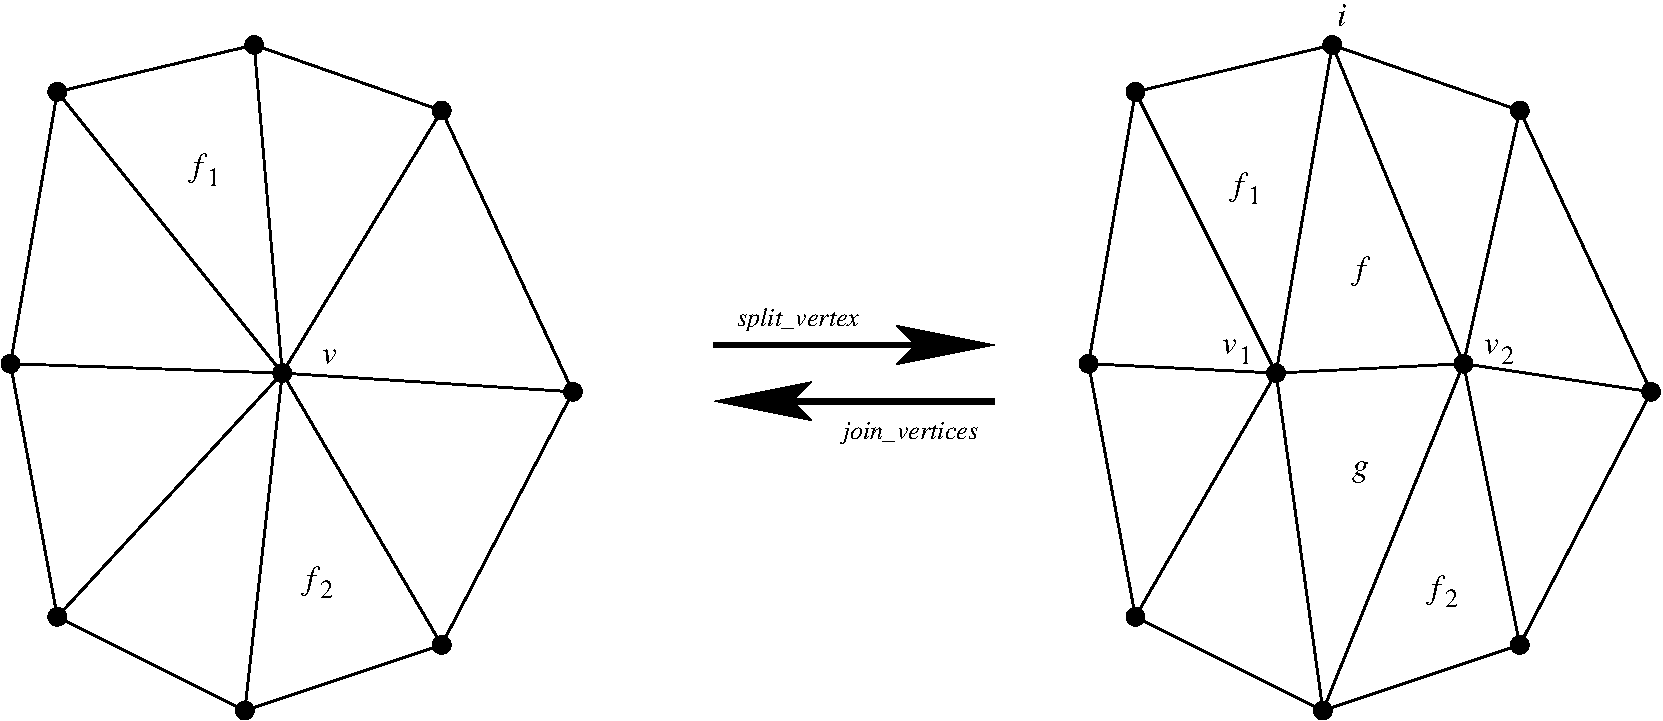
\includegraphics[width=0.9\textwidth]{TDS_2_ref/join_split}
\end{center}
\end{ccTexOnly}
\begin{ccHtmlOnly}
<center>
<img border=0 src="./join_split.gif" align=center
alt="The join and split operations"
title="The join and split operations">
</center>
\end{ccHtmlOnly}
\begin{ccHtmlOnly}
<br><font size=-1>
\end{ccHtmlOnly}
\caption{The join and split operations.}\label{fig-tds-split-join}
%Left to right:
%The vertex \ccc{v} is split into $v_1$ and $v_2$. The faces $f$ and
%$g$ are inserted after $f_1$ and $f_2$, respectively, in the
%counter-clockwise sense. The vertices $v_1$, $v_2$ and the faces $f$
%and $g$ are returned as a \ccc{boost} \ccc{tuple} in that order.
%Right to left: The edge \ccc{(f,i)} is collapsed, and thus the
%vertices $v_1$ and $v_2$ are joined. The vertex \ccc{v} is
%returned.}
\begin{ccHtmlOnly}
</font>
\end{ccHtmlOnly}
\end{figure}

\begin{figure}[htb]
\begin{ccTexOnly}
\begin{center}
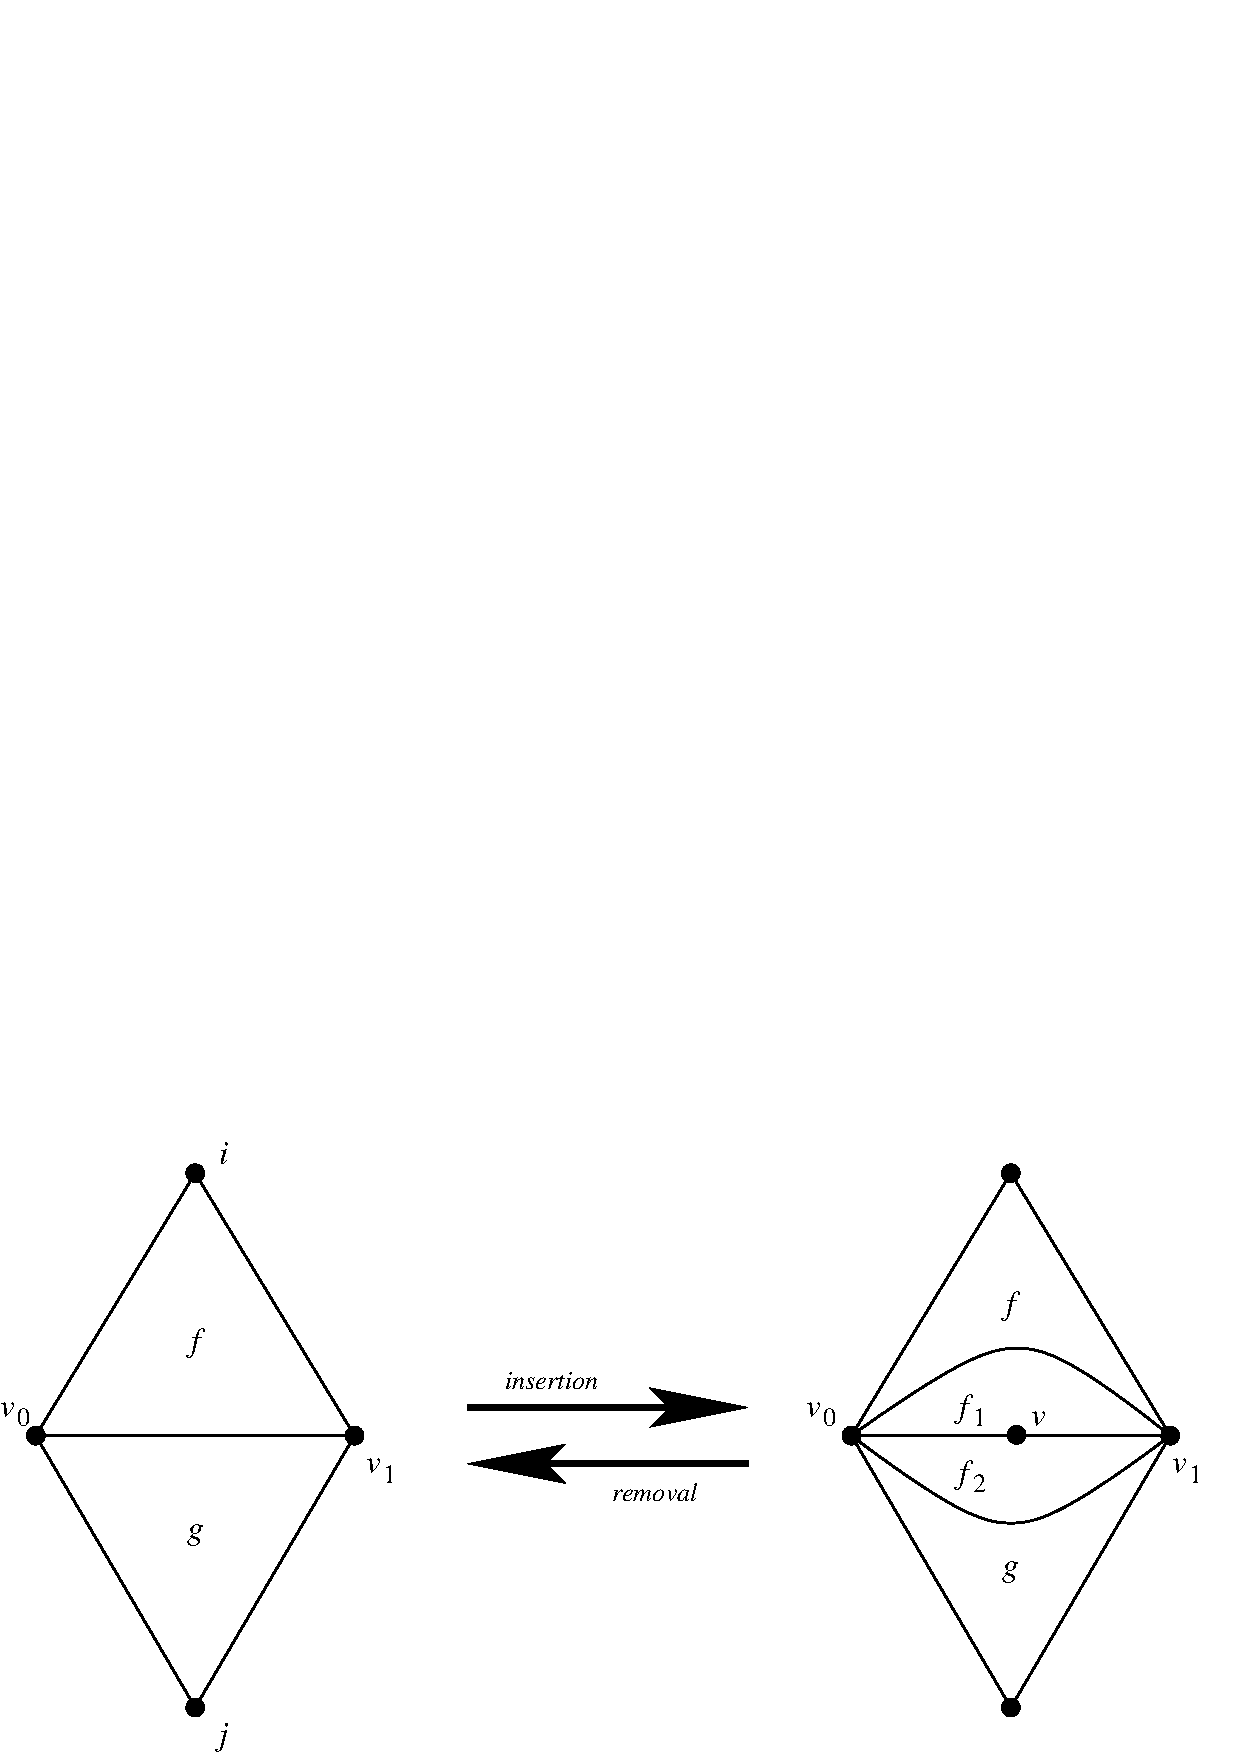
\includegraphics[width=0.8\textwidth]{TDS_2_ref/tds-insert_degree_2}
\end{center}
\end{ccTexOnly}
\begin{ccHtmlOnly}
<center>
<img border=0 src="./tds-insert_degree_2.gif" align=center
alt="Insertion and removal of degree 2 vertices"
title="Insertion and removal of degree 2 vertices">
</center>
\end{ccHtmlOnly}
\begin{ccHtmlOnly}
<br><font size=-1>
\end{ccHtmlOnly}
\caption{Insertion and removal of degree 2 vertices.}
%Left to right:
%The edge \ccc{(f,i)} is replaced by two edges by means of inserting a
%vertex \ccc{v} on the edge. The faces $f_1$ and $f_2$ are
%created. Right to left: the faces $f_1$ and $f_2$ are
%destroyed. The vertex \ccc{v} is deleted and its two adjacent edges
%are merged.}
\label{fig-tds-ir-deg2}
\begin{ccHtmlOnly}
</font>
\end{ccHtmlOnly}
\end{figure}



\end{ccRefClass}

% +------------------------------------------------------------------------+
%%RefPage: end of main body, begin of footer
% EOF
% +------------------------------------------------------------------------+

